\documentclass{article}

% if you need to pass options to natbib, use, e.g.:
%     \PassOptionsToPackage{numbers, compress}{natbib}
% before loading neurips_2020

% ready for submission
% \usepackage{neurips_2020}

% to compile a preprint version, e.g., for submission to arXiv, add add the
% [preprint] option:
%     \usepackage[preprint]{neurips_2020}

% to compile a camera-ready version, add the [final] option, e.g.:
%     \usepackage[final]{neurips_2020}

% to avoid loading the natbib package, add option nonatbib:
\usepackage[nonatbib]{neurips_2020}

\usepackage[utf8]{inputenc} % allow utf-8 input
\usepackage[T1]{fontenc}    % use 8-bit T1 fonts
\usepackage{hyperref}       % hyperlinks
\usepackage{url}            % simple URL typesetting
\usepackage{booktabs}       % professional-quality tables
\usepackage{amsfonts}       % blackboard math symbols
\usepackage{nicefrac}       % compact symbols for 1/2, etc.
\usepackage{microtype}      % microtypography


%%%%我的包
\usepackage{graphicx}
%\graphicspath{ {./images/} }
\usepackage{float} 
\title{Report of face-recognition by finetuning \\ ResNet and Haorui-Net}
\documentclass{article}
\usepackage[utf8]{inputenc}
\usepackage{booktabs} %三线表需要加载宏包{booktabs}
\usepackage{diagbox}
\usepackage{multirow}
\usepackage{listings}
\usepackage{xcolor}

%New colors defined below
\definecolor{codegreen}{rgb}{0,0.6,0}
\definecolor{codegray}{rgb}{0.5,0.5,0.5}
\definecolor{codepurple}{rgb}{0.58,0,0.82}
\definecolor{backcolour}{rgb}{0.95,0.95,0.92}

%Code listing style named "mystyle"
\lstdefinestyle{mystyle}{
  backgroundcolor=\color{backcolour},   commentstyle=\color{codegreen},
  keywordstyle=\color{magenta},
  numberstyle=\tiny\color{codegray},
  stringstyle=\color{codepurple},
  basicstyle=\ttfamily\footnotesize,
  breakatwhitespace=false,         
  breaklines=true,                 
  captionpos=b,                    
  keepspaces=true,                 
  numbers=left,                    
  numbersep=5pt,                  
  showspaces=false,                
  showstringspaces=false,
  showtabs=false,                  
  tabsize=2
}

%"mystyle" code listing set
\lstset{style=mystyle}



% The \author macro works with any number of authors. There are two commands
% used to separate the names and addresses of multiple authors: \And and \AND.
%
% Using \And between authors leaves it to LaTeX to determine where to break the
% lines. Using \AND forces a line break at that point. So, if LaTeX puts 3 of 4
% authors names on the first line, and the last on the second line, try using
% \AND instead of \And before the third author name.

\author{
   Haorui Li\thanks \\
  Chien-Shiung Wu College\\
  Southeast University\\
  % examples of more authors
  % \And
  % Coauthor \\
  % Affiliation \\
  % Address \\
  % \texttt{email} \\
  % \AND
  % Coauthor \\
  % Affiliation \\
  % Address \\
  % \texttt{email} \\
  % \And
  % Coauthor \\
  % Affiliation \\
  % Address \\
  % \texttt{email} \\
  % \And
  % Coauthor \\
  % Affiliation \\
  % Address \\
  % \texttt{email} \\
}

\begin{document}

\maketitle

\begin{abstract}
For face recognition, first, I use MTCNN and face.evoLVe for automatic data cleansing, then rename the folders by batch processing in order to fit the requirenments of Dataset.ImageFolder. Third, I trained two modles for face recognition, one is self-modified Resnet, another is InceptionResNetV1 with pre-trained weight, and finetuning the modle on classmates' data. Finally the best cross-entropy loss is 0.1830 and recognize 82/104 classmates.  
\end{abstract}

\section{Data prepare}
\subsection{Face alignment}
To begin with, I use MTCNN[1] and \textit{face.evoLVe.PyTorch} for automatic face alignment.

MTCNN propose a deep cascaded multi-task framework which
exploits the inherent correlation between them to boost up Resnet's performance on face alignment, the architecture is as follows:
\begin{figure}[H]%H为当前位置,!htb为忽略美学标准,htbp为浮动图形
  \centering
  \caption{MTCNN's architecture}
%可选参数中width=\columnwidth选取了当前列宽
  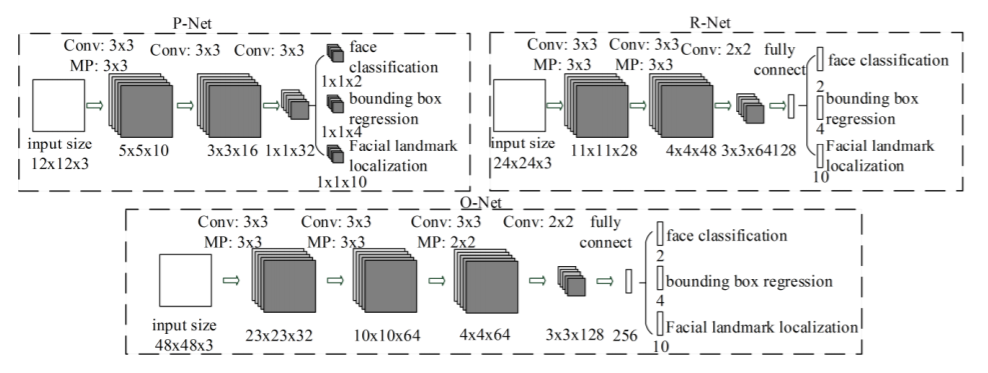
\includegraphics[width=\columnwidth]{IMG/MTCNN.png} %插入图片,[]中设置图片大小,{}中是图片文件名
  \label{Fig.RNN} %用于文内引用的标签
\end{figure}
Though MTCNN is very fast, but it sometimes go wrong and bring in dirty data, like the Figure2, and these dirty data will definitely bring catastrophe for model trainning.
\begin{figure}[H]%H为当前位置,!htb为忽略美学标准,htbp为浮动图形
  \centering
  \caption{Samples of dirty data by MTCNN}
%可选参数中width=\columnwidth选取了当前列宽
  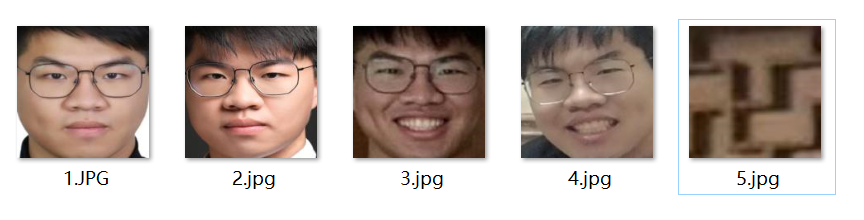
\includegraphics[width=\columnwidth]{IMG/ML大作业筛选展示.png} %插入图片,[]中设置图片大小,{}中是图片文件名
  \label{Fig.RNN} %用于文内引用的标签
\end{figure}
So I refer to \textit{face.evoLVe's face-align tools} and finally get good data.
This tool can be find at:
\begin{center}
  \url{https://github.com/ZhaoJ9014/face.evoLVe.PyTorch}
\end{center}
This tool is about 4-times slower than MTCNN, but brings no dirty data.
\subsection{Rebuild folder architecture}
For quick detect image labels, I use \textit{torchvision.datasets.ImageFolder} to automatically read classmates name. To use this function, I rebuild the data folder's architecture by code.

Exactly, I use os.rename and string.split. Following are some codes I use to split the student number:

\begin{lstlisting}[language=Python, caption=Change folder names for ImageFloder function]
def replaceDirName(rootDir):
  #Change the folders' name under rootDir, split the student number by '-' or '_'
    num = 0
    dirs = os.listdir(rootDir)
    for dir in dirs:
        print('oldname is:' + dir)
        num = num +1
        try:
          temp = dir.split('_')[1]
        except IndexError:
          try:
            temp=dir.split('-')[1]
          except:
            print("This is not Number-Name structure", dir)
            continue
        except:
          print("This is not - or _ structure", dir)
          continue
        print('new name:',temp)
        oldname = os.path.join(rootDir, dir)
        newname = os.path.join(rootDir, temp)
        os.rename(oldname, newname)#replace
replaceDirName('align_data')
\end{lstlisting}




After rebuild the folder architecture, \textit{torchvision.datasets.ImageFolder} is able to automatically read sub-folders' name as image label. 

\subsection{Transforms}
After clean the data and align all the faces, I made some extra preparations for models robustness and these work has brought about 3-point increase in test accuracy.

When load in the data I perform some random transforms to the images to improve training. Different transforms can be attempted and I tried various ones, like Random-Color-Jitter and Random-Rotation, along with Random-Horizontal-Flip.
\begin{figure}[H]%H为当前位置,!htb为忽略美学标准,htbp为浮动图形
  \centering
  \caption{Examples of random Color Jitter}
%可选参数中width=\columnwidth选取了当前列宽
  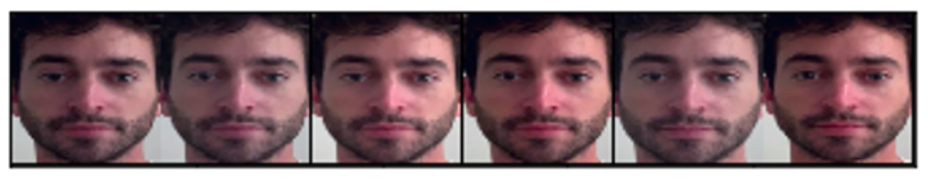
\includegraphics[width=\columnwidth]{IMG/随机彩色.png} %插入图片,[]中设置图片大小,{}中是图片文件名
  \label{Fig.RNN} %用于文内引用的标签
\end{figure}
Finally I choose all these transforms to improve the model's robustness. And the random-color-jitter improves about 2 points in accuracy probably because classmates take photo at different light environment.

\section{Design model architecture}
Due to the fact that the data we have is small scale, it will be hard to train a model without over-fitting. So I think it is recognized to use some pre-trained model and do the fine-tuning.  What I have to do is design the final layers.

\subsection{Pre-trained ResNet}
The pre-trained weight I download is the Facenet trained by Google. They use triple loss and finally get 0.997 accuracy at Lwf, the High-Level modal structure of Facenet is as follow[2]:
\begin{figure}[H]%H为当前位置,!htb为忽略美学标准,htbp为浮动图形
  \centering
  \caption{High Level Modal Structure of Facenet}
%可选参数中width=\columnwidth选取了当前列宽
  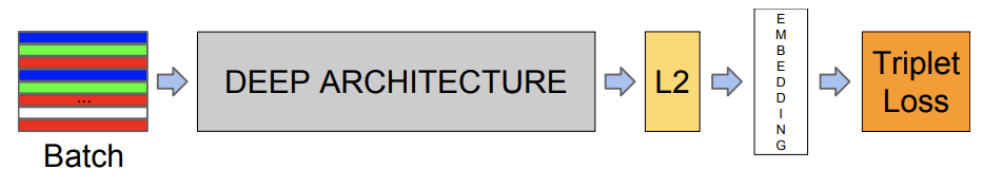
\includegraphics[width=\columnwidth]{IMG/facenet.png} %插入图片,[]中设置图片大小,{}中是图片文件名
  \label{Fig.RNN} %用于文内引用的标签
\end{figure}
And for the first model, I use Inception-ResNet[3] to fine-tuning the model, which is designed for fine-tuning Facenet. The architecture of Inception-ResNet is as follow:
\begin{figure}[H]%H为当前位置,!htb为忽略美学标准,htbp为浮动图形
  \centering
  \caption{Inception-ResNet}
%可选参数中width=\columnwidth选取了当前列宽
  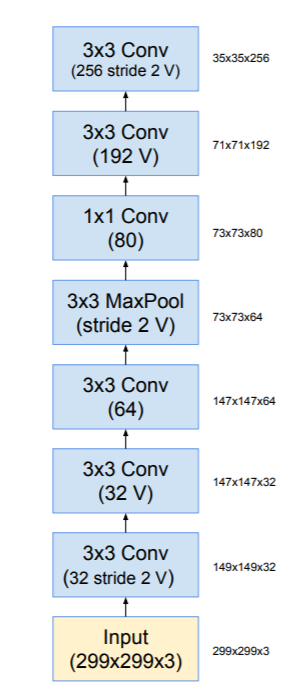
\includegraphics[width=18ex]{IMG/RESNET.png} %插入图片,[]中设置图片大小,{}中是图片文件名
  \label{Fig.RNN} %用于文内引用的标签
\end{figure}
The code of final layers are:
\begin{lstlisting}[language=Python, caption=Final layer Codes]
        self.block8 = Block8(noReLU=True)
        self.avgpool_1a = nn.AdaptiveAvgPool2d(1)
        self.dropout = nn.Dropout(dropout_prob)
        self.last_linear = nn.Linear(1792, 512, bias=False)
        self.last_bn = nn.BatchNorm1d(512, eps=0.001, momentum=0.1, affine=True)
        self.logits = nn.Linear(512, tmp_classes)
\end{lstlisting}
And I have modified the final layers to test which model is best.

\subsection{Modified ResNet}
From the upper section we can see the final six layers are:
\begin{lstlisting}[language=Python, caption=Final layers]
[Block8(
   (branch0): BasicConv2d(
     (conv): Conv2d(1792, 192, kernel_size=(1, 1), stride=(1, 1), bias=False)
     (bn): BatchNorm2d(192, eps=0.001, momentum=0.1, affine=True, track_running_stats=True)
     (relu): ReLU()
   )
   (branch1): Sequential(
     (0): BasicConv2d(
       (conv): Conv2d(1792, 192, kernel_size=(1, 1), stride=(1, 1), bias=False)
       (bn): BatchNorm2d(192, eps=0.001, momentum=0.1, affine=True, track_running_stats=True)
       (relu): ReLU()
     )
     (1): BasicConv2d(
       (conv): Conv2d(192, 192, kernel_size=(1, 3), stride=(1, 1), padding=(0, 1), bias=False)
       (bn): BatchNorm2d(192, eps=0.001, momentum=0.1, affine=True, track_running_stats=True)
       (relu): ReLU()
     )
     (2): BasicConv2d(
       (conv): Conv2d(192, 192, kernel_size=(3, 1), stride=(1, 1), padding=(1, 0), bias=False)
       (bn): BatchNorm2d(192, eps=0.001, momentum=0.1, affine=True, track_running_stats=True)
       (relu): ReLU()
     )
   )
   (conv2d): Conv2d(384, 1792, kernel_size=(1, 1), stride=(1, 1))
 ),
 AdaptiveAvgPool2d(output_size=1),
 Linear(in_features=1792, out_features=512, bias=False),
 BatchNorm1d(512, eps=0.001, momentum=0.1, affine=True, track_running_stats=True),
 Linear(in_features=512, out_features=8631, bias=True),
 Softmax(dim=1)]
\end{lstlisting}
Because earlier layers as containing the base-level information needed to recognize face attributes and base level characteristics, so I want to cut the layers after Conv2d and use some my own code, and just updating the final layers to include another 104 faces.

Put all beginning layers in an nn.Sequential:
\begin{lstlisting}[language=Python, caption=Keep the conv2d layers]
model_ft = nn.Sequential(*list(model_ft.children())[:-5])
\end{lstlisting}
Now, model modified is a torch model but without the final linear, pooling, batchnorm, and sigmoid layers.

After this, I design another final layers calss includs Flatten and Normalize, the codes are:
\begin{lstlisting}[language=Python, caption=Haorui Net]
#Change the final layers as follows
model_modified.avgpool_1a = nn.AdaptiveAvgPool2d(output_size=1)
model_modified.last_linear = nn.Sequential(
    Flatten(),
    nn.Linear(in_features=1792, out_features=512, bias=False),
    normalize()
)
model_modified.logits = nn.Linear(layer_list[4].in_features,104)
model_modified.softmax = nn.Softmax(dim=1)
model_modified = model_modified.to(device)
\end{lstlisting}
So the architecture is:
\begin{figure}[H]%H为当前位置,!htb为忽略美学标准,htbp为浮动图形
  \centering
  \caption{Haorui-Net Architecture}
%可选参数中width=\columnwidth选取了当前列宽
  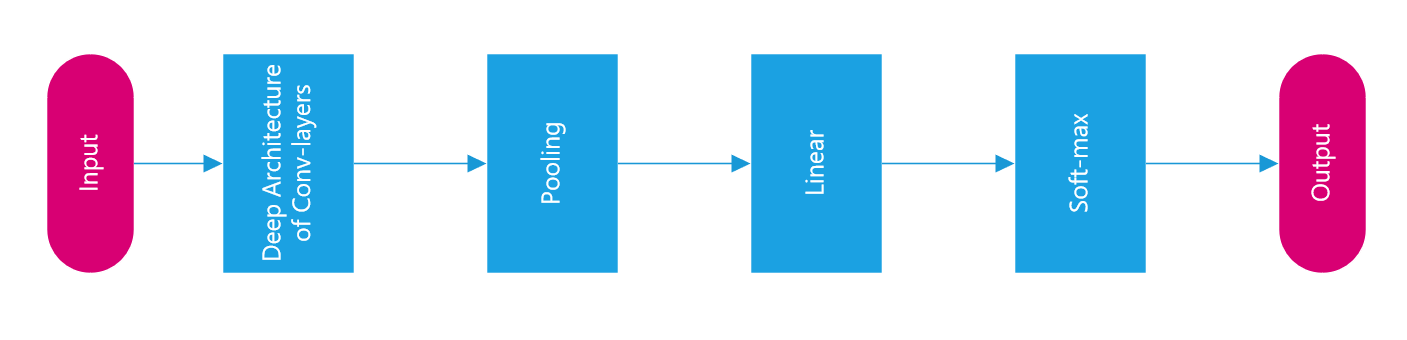
\includegraphics[width=\columnwidth]{IMG/haoruinet.png} %插入图片,[]中设置图片大小,{}中是图片文件名
  \label{Fig.RNN} %用于文内引用的标签
\end{figure}

We can name it Haorui-ResNet. In the next section I will train these two models and show some details to pick the winner.

\section{Training and preferences}
After design the model, I begin the training step. Tried different epoch, batch size, learning rate and models.

The options of batch size are often limited by GPU memory.

On my machine, I have a  single Tesla-P-100 with 16280 MiB memory, which means I have more choice on batch size and epochs. 

Use '!nvidia-smi' I get the following in formations of GPU memeory, it shows that 6869 MiB memory is located at device and I still have space to test. 
\begin{figure}[H]%H为当前位置,!htb为忽略美学标准,htbp为浮动图形
  \centering
  \caption{24 Epochs and 64 Batch-size}
%可选参数中width=\columnwidth选取了当前列宽
  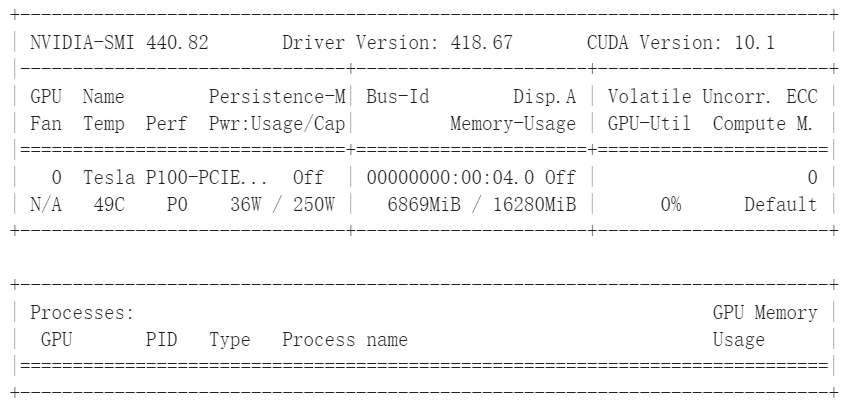
\includegraphics[width=\columnwidth]{IMG/ML实验GPU.png} %插入图片,[]中设置图片大小,{}中是图片文件名
  \label{Fig.RNN} %用于文内引用的标签
\end{figure}
After choose several combinations of epochs and batch size,  I get the results as follows on Inception-ResNet:

\begin{table}[!htbp]
\centering
\caption{Records of combination for ResNet}\label{tab:aStrangeTable}%添加标题 设置标签
\begin{tabular}{cccc}
\toprule
Epochs & Batch size& TP &Train FPS\\
\midrule
10& 16 & 21 & 427.4\\
24& 16& 26 & 420.7\\
24 & 32 & 41 & 279.6\\
24 & 64 & 75 & 153.4\\
32 & 64 & 71 & 161.5\\
24 & 128 & 80 & 149.5\\
32 & 128 & 77 & 233.9\\
24 & 256 & 70  &183.3\\
32 & 256 & 77  &192.8\\
64 & 256 & 76  &155.3\\
\bottomrule
\end{tabular}

%\caption{这是一张三线表}\label{tab:aStrangeTable}  标题放在这里也是可以的
\end{table}
From the chart we can see, more batch size often means better performance, but with more batch size, sometimes it need more epochs to minimize the loss, just like 256 batch size performs weaker than 128 batch size in 24 epochs, and become better in 32 epochs.

So finally, the ResNet performs its best at 24 epochs, 128 batch size and reaches 82 true positive. This model was saved as  '24-epoch-128bz-VGGFACE2-TEST80ACC.pb'.

With the chart above, I can qiuckly choose some combinations for Haorui-Net, and the results are as follows:

\begin{table}[!htbp]
\centering
\caption{Records of combination for Haorui-Net}\label{tab:aStrangeTable}%添加标题 设置标签
\begin{tabular}{cccc}
\toprule
Epochs & Batch size& TP &Train FPS\\
\midrule
24 & 128 & 82 & 171.4\\
32 & 128 & 76 & 255.5\\
\bottomrule
\end{tabular}
\end{table}

Luckily, the Haorui-Net performs better than ResNet its best at 24 epochs, 128 batch size and reaches 82 true positive. This model was saved as  '24-epoch-128bz-MODIFIED-TEST82ACC.pb'.

So I'm proud to announce that Haorui-Net becomes the winner in this combination, with two more ture-positive!

But what I want to point out is that, Haorui-Net is weaker in the decrease of loss, for ResNet, the minimum of loss is about 0.27 while training, but for Haorui-Net, the minimum loss is about 3.8, it probably means ResNet is designed more smarter in track and reduce the loss.

\section{Conclusion}



%%%%%%%%%%%%%%%%%%%%%%%%%%%%%%%%
%%%%%%%%%%%%%%%%%%%%%%%%%%%%%%%%
%%%%%%%%%%%%%%%%%%%%%%%%%%%%%%%%

\section*{References}


\medskip

\small

[1] Zhang, K., Zhang, Z., Li, Z. & Qiao, Y. (2016). Joint Face Detection and Alignment using Multi-task Cascaded Convolutional Networks.. CoRR, abs/1604.02878.

[2]Schroff, F., Kalenichenko, D. & Philbin, J. (2015). FaceNet: A Unified Embedding for Face Recognition and Clustering (cite arxiv:1503.03832Comment: Also published, in Proceedings of the IEEE Computer Society Conference on Computer Vision and Pattern Recognition 2015)

[3]Szegedy, C., Ioffe, S., Vanhoucke, V. & Alemi, A. A. (2017). Inception-v4, Inception-ResNet and the Impact of Residual Connections on Learning. Proceedings of the 31st AAAI Conference on Artificial Intelligence (p./pp. 4278--4284), : AAAI Press.




\end{document}
